\documentclass{beamer}
\usepackage{ulem}
\usetheme{Dresden}
\usecolortheme{wolverine}

\title{Tube Room Update}
\author{Evan Carpenter}
\setbeamertemplate{navigation symbols}{}
\addtobeamertemplate{navigation symbols}{}{%
    \usebeamerfont{footline}%
    \usebeamercolor[fg]{footline}%
    \hspace{1em}%
    \insertframenumber/4
}

\begin{document}
\titlepage
\section{Delivery Updates}
	\begin{frame}
		\begin{block}{Delivery:}
			\begin{itemize}
				\item \small MSU delivered 150 tubes last Friday. 0 Bent. 
				\item Next delivery is this Thursday Jan 26th.
			\end{itemize}
		\end{block}	
		\begin{block}{Tube Testing:}
			\begin{itemize}
				\item MSU's Leak detector is up and running! Reinhard says it has been working since December. 
				\item Mod 37 and 38 are ready and covered in Tube Room. 
				\item There are enough good tubes for Mod 39.
				\item Only 155 MSU tubes from different dates still need leak test. 
				\item Lots of tension and leak tests were done in the past week, many new tubes are now ready. 
			\end{itemize}
		\end{block}
	\end{frame}


\section{Tube Room Inventory}
	\subsection{MSU Tubes}
		\begin{frame}{MSU Tubes}
			\scalebox{0.6}{
			\begin{tabular}{|c|c|c|c|c|c|c|c|c|c|c|c|}
				\hline
				WeekDate & MSU &BENT& Lok& Tok & T2ok& DCok& DONE&  OK  &GONE&USED &READY\\\hline
				10/28/22 & 503 & 0 & 503 & 492 & 469 & 496 & 483 & 465 & 11 & 354 & 111\\
                11/04/22 & 100 & 1 & 100 & 100 &  88 & 100 &  99 &  88 &  0 &  10 &  78\\
                11/18/22 & 200 & 0 & 200 & 199 & 183 & 200 & 198 & 183 &  1 &   9 & 174\\
                11/25/22 & 300 & 0 & 300 & 298 & 255 & 299 & 275 & 254 &  2 &   0 & 254\\
                12/02/22 & 195 & 0 & 195 & 194 & 163 & 195 & 177 & 163 &  1 &   0 & 163\\
                12/09/22 & 100 & 2 & 100 & 100 &  90 &  99 &  97 &  90 &  0 &   0 &  90\\
                01/06/23 & 200 & 0 & 200 & 198 & 188 & 197 & 199 & 185 &  2 &   0 & 185\\
                01/13/23 & 200 & 5 & 195 & 199 & 181 & 198 & 193 & 181 &  1 &   0 & 181\\
                01/20/23 & 150 & 0 & 0 & 150 &   0 &   0 &   0 &   0 &  0 &   0 &   0\\\hline
														
				TOTAL &    1948& 8 &1948 &1930&1617&1784	&1721	&1609	&18	&373	&1236\\\hline
			\end{tabular}}
			\vspace{0.5cm}
			\begin{itemize}
				\item 150 tubes from new shipment have not been leak tested yet. 
				\item This total is including Mod 37, 38. 
			\end{itemize}
		\end{frame}
	\subsection{UM Tubes}
		\begin{frame}{UM Tubes}
			\scalebox{0.6}{
			\begin{tabular}{|c|c|c|c|c|c|c|c|c|c|c|c|}
				\hline
				WeekDate & UM &BENT& Lok& Tok & T2ok& DCok& DONE&  OK  &GONE&USED &READY\\\hline
				11/04/22 & 129 & 1 & 129 & 127 & 126 & 128 & 127 & 124 & 4 &  84 &  40\\
				11/11/22 & 233 & 1 & 232 & 231 & 227 & 230 & 226 & 223 & 3 & 142 &  81\\
				11/18/22 & 260 & 4 & 260 & 259 & 255 & 258 & 256 & 253 & 1 & 173 &  80\\
				11/25/22 & 101 & 0 & 100 & 101 & 100 & 100 & 100 & 100 & 0 &  61 &  39\\
				12/02/22 & 250 & 0 & 250 & 249 & 249 & 250 & 249 & 248 & 1 & 101 & 147\\
				12/09/22 & 191 & 2 & 191 & 188 & 184 & 188 & 186 & 183 & 2 &   0 & 183\\
				12/16/22 & 188 & 1 & 188 & 188 & 185 & 186 & 185 & 185 & 0 &   0 & 185\\\hline
				TOTAL &1352&	9&	1350&	1343&	1326&	1340&	1329&	1316&	11&	561&	755\\\hline
			\end{tabular}}
			\begin{itemize}
				\item 1,236 MSU Tubes + 755 UM Tubes = \textbf{1,991 Total Ready}
				\item Accounting for Mod 37 and 38: $$1,991-464-464={\bf 1,063\ Ready\ \text{After 37, 38}}$$
				\item Rough manual count showed $\sim1,050$ good, so this number should be accurate.
				\item More sorting needs to be done to check T2 status.
			\end{itemize}
			
		\end{frame}
	

		\begin{frame}
			%\frametitle{Tube Room Inventory - UM Tubes}
			\begin{figure}
				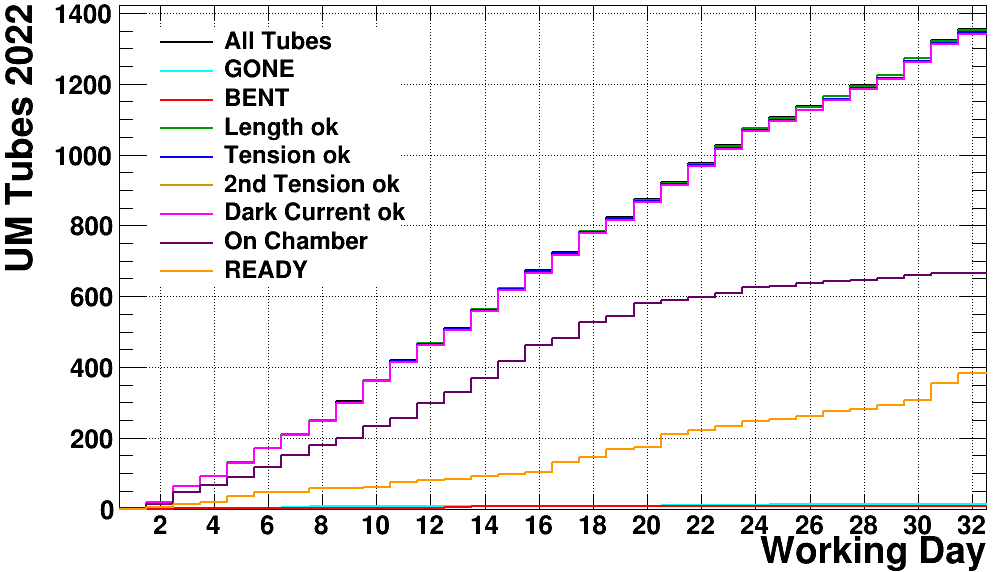
\includegraphics[width=\linewidth]{UMdaily2022.png}
			\end{figure}
		\end{frame}
\section*{Backup Slides}
	\appendix
	\begin{frame}
		Tests of automating summary-making process.
	\end{frame}
	\begin{frame}{Tube Room Inventory - MSU Tubes}
		\begin{figure}
			\centering
			\scalebox{0.6}{\begin{tabular}{r|r|r|r|r|r|r|r|r|r|r}
\toprule
           Received &  MSU &  Lost &  Bent &  LT$_\text{ok}$ &  T1$_\text{ok}$ &  T2$_\text{ok}$ &  DC$_\text{ok}$ &  Passed All &  In Chamber &  Ready \\
\midrule
(UM tubes this row) & 1359 &    19 &     9 &            1359 &            1343 &            1351 &            1353 &        1329 &        1038 &    291 \\
         2022-10-28 &  503 &    13 &    13 &             503 &             492 &             494 &             502 &         478 &         431 &     47 \\
         2022-11-04 &  100 &     1 &     1 &             100 &             100 &             100 &             100 &          99 &          81 &     18 \\
         2022-11-18 &  200 &     1 &     0 &             200 &             198 &             199 &             200 &         198 &         171 &     27 \\
         2022-11-25 &  302 &    22 &    22 &             302 &             300 &             298 &             302 &         278 &         206 &     72 \\
         2022-12-02 &  195 &    16 &    14 &             195 &             192 &             191 &             195 &         178 &         105 &     73 \\
         2022-12-09 &  100 &     3 &     2 &             100 &             100 &             100 &             100 &          97 &          66 &     31 \\
         2023-01-06 &  200 &     1 &     0 &             200 &             197 &             199 &             200 &         197 &         108 &     89 \\
         2023-01-13 &  200 &     6 &     5 &             200 &             200 &             200 &             200 &         194 &         114 &     80 \\
         2023-01-20 &  150 &     1 &     0 &             150 &             147 &             148 &             150 &         146 &           5 &    141 \\
         2023-01-27 &  100 &     0 &     0 &             100 &             100 &             100 &             100 &         100 &           0 &    100 \\
         2023-02-03 &  199 &     2 &     0 &             199 &             198 &             196 &             199 &         195 &           0 &    195 \\
         2023-02-10 &  192 &     2 &     2 &             192 &             189 &             182 &             192 &         180 &           0 &    180 \\
         2023-03-17 &  849 &     2 &     0 &             849 &             846 &             218 &             342 &         215 &           0 &    215 \\
              Total & 4649 &    89 &    68 &            4649 &            4602 &            3976 &            4135 &        3884 &        2325 &   1559 \\
\bottomrule
\end{tabular}
}
			\caption{Currently there is no way to keep track of individual dates' leak tests. I subtract it at the end so the total number of ``Ready'' tubes is accurate.}
		\end{figure}
		\centering
		%Potential Good MSU Tubes: \\
		%Total Potential Good:
	\end{frame}
\end{document}


 10/28/22 &   2 & 0 &   2 &   2 &   1 &   2 &   1 &   1 & 0 &  0 &   1
 11/04/22 & 129 & 1 & 129 & 127 &  72 & 122 &  72 &  70 & 3 & 31 &  39
 11/11/22 & 233 & 1 & 232 & 232 & 144 & 230 & 144 & 142 & 2 & 54 &  88
 11/18/22 & 260 & 4 & 260 & 259 & 174 & 258 & 174 & 173 & 1 & 37 & 136
 11/25/22 & 101 & 0 & 100 & 101 &  61 & 100 &  61 &  61 & 0 &  2 &  59
 12/02/22 & 250 & 0 & 250 & 245 & 138 & 250 & 138 & 138 & 1 & 31 & 107
 12/09/22 & 191 & 0 & 191 & 188 &   0 & 188 &   0 &   0 & 1 &  0 &   0
 12/16/22 & 188 & 0 & 188 & 188 &   0 & 132 &   0 &   0 & 0 &  0 &   0